\ProvidesFile{Q23.tex}[Билет 23]

\section{Билет 23. Сформулируйте теорему Каруша-Куна-Таккера. Объясните, в чём смысл условий дополняющей нежёсткости?}
\textit{Мотивация.} Помимо задач с ограничениями типа равенств, часто встречаются задачи с ограничениями типа неравенств.
Например, вместо окружности $x^2 + y^2 = 1$ нужно исследовать круг $x^2 + y^2 \leqslant 1$. Такие задачи называются задачами
нелинейного программирования. Пусть $x = (x_1, \, ..., \, x_n) \in \mathbb{R}^n$, тогда сформулируем задачу:
\[\left\{\begin{aligned}
    &f(x) \to extr \\
    &g_i(x) \leqslant 0, \, i = 1, \,..., \, m \text{ ($m$ может быть больше $n$)}
\end{aligned}\right.\]

\textbf{Пример.}
\[\left\{\begin{aligned}
    &f(x, \, y) \to extr \\
    &g_1(x, y) = x^2 + y^2 - 1 \leqslant 0 \\
    &g_2(x, y) = -x - y \leqslant 0
\end{aligned}\right.\]

\begin{figure}[h]
    \begin{center}
        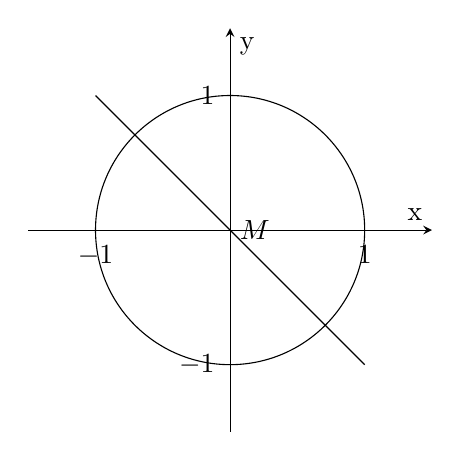
\begin{tikzpicture}
            \begin{axis}[xlabel={x}, ylabel={y}, xmin=-1.5, xmax=1.5, ymin=-1.5, ymax=1.5, axis lines = center, width=5cm, height=5cm, scale=1.5]
                \draw[black] (0, 0) circle [radius = 1] node[right] {$M$};
                \draw[domain = -1:1] plot(\x, -\x);
            \end{axis}
        \end{tikzpicture}
    \end{center}
\end{figure}

Пусть $M$ -- множество, которое задаётся ограничениями $g_i$. Разбор случаев (при помощи метода множителей Лагранжа):
\begin{enumerate}
    \item Кандидатов в точки экстремума внутри M:
        \[\left\{\begin{aligned}
            f^{'}_x = 0 \\
            f^{'}_y = 0 \\
            g_1 < 0 \\
            g_2 < 0
        \end{aligned}\right.\]
    \item Кандидаты на дуге окружности:
        \[\left\{\begin{aligned}
            f^{'}_x - \lambda_1 (g_1)^{'}_x = 0 \\
            f^{'}_y - \lambda_1 (g_2)^{'}_y = 0 \\
            g_1 = 0 \\
            g_2 < 0
        \end{aligned}\right.\]
    \item Кандидаты на отрезке внутри круга:
        \[\left\{\begin{aligned}
            f^{'}_x - \lambda_2 (g_2)^{'}_x = 0 \\
            f^{'}_y - \lambda_2 (g_2)^{'}_y = 0 \\
            g_2 = 0 \\
            g_1 < 0
        \end{aligned}\right.\]
    \item Кандидаты на пересечении окружности и прямой:
        \[\left\{\begin{aligned}
            f^{'}_x - \lambda_1 (g_1)^{'}_x - \lambda_2 (g_2)^{'}_x = 0 \\
            f^{'}_y - \lambda_1 (g_1)^{'}_y - \lambda_2 (g_2)^{'}_y = 0 \\
            g_1 = 0 \\
            g_2 = 0
        \end{aligned}\right.\]
\end{enumerate}
Далее во всех полученных кандидатах вычисляем целевую функцию.

\begin{theorem}{\textbf{Каруша-Куна-Таккера (простая версия для задачи с ограничениями типа неравенств).}}
Допустим, что $x^{(0)}$ -- решение задачи
$\begin{cases}
    f(x) \to extr \\
    g_i(x) \leqslant 0, i = 1, ..., m
\end{cases}$\\
Пусть $L(x, \lambda) = f(x) - \sum\limits_{i = 1}^{m} \lambda_i g_i(x)$ -- функция Лагранжа. Тогда в точке $x^{(0)}$ выполнено:
\[\left\{\begin{aligned}
    L^{'}_{x_j} &= 0, j = 1, ..., n\\
    g_i(x) &\leqslant 0, i = 1, ..., m\\
    \lambda_i g_i(x) &= 0, i = 1, ..., m \text{ -- условия дополняющей нежёсткости}
\end{aligned}\right.\]
\end{theorem}

\begin{remark}
В чём смысл условий дополняющей нежёсткости?
\end{remark}